\documentclass[11pt]{article}

% Any percent sign marks a comment to the end of the line

% Every latex document starts with a documentclass declaration like this
% The option dvips allows for graphics, 12pt is the font size, and article
%   is the style

\usepackage[pdftex]{graphicx}
\usepackage{url}

\usepackage{soul}

\usepackage{graphicx} % Required for including images

\usepackage{setspace}
\setstretch{0.85}


%\usepackage{geometry}
% \geometry{
% left=7.6cm,top=0.1cm,right=1cm,bottom=0.1cm,nohead,nofoot
% }

% These are additional packages for "pdflatex", graphics, and to include
% hyperlinks inside a document.

\setlength{\oddsidemargin}{-0.25in}
\setlength{\textwidth}{7in}
\setlength{\topmargin}{-0.8in}
\setlength{\textheight}{9.2in}

% These force using more of the margins that is the default style

\begin{document}

% Everything after this becomes content
% Replace the text between curly brackets with your own

%\title{Hong Kong Labour Market Data Visualization}
%\author{Fong Chun Him (3035377115), Wu Szu Han (3035562617)}
%\date{November 17, 2020}

% You can leave out "date" and it will be added automatically for today
% You can change the "\today" date to any text you like


%\maketitle

% This command causes the title to be created in the document

\begin{center}
\huge{Short proposal for Gmail scam detector plug-in}
\end{center}

\section*{\large{1 \hspace{10pt} Gmail email client is chosen}}
\begin{enumerate}
\item \textbf{Popularity}: Consider Email Client Market Share in 2020, Gmail email client is 38\% and Apple Mail email client is 40\%. Besides, Gmail is by far the most popular browser email client.
\item \textbf{Public REST API}: Gmail API is public whereas Apple Mail API is private.
\end{enumerate}

\section*{\large{2 \hspace{10pt} Other choices}}

\begin{spacing}{1}

\begin{center}
 \begin{tabular}{|c | c|} 
 \hline
 Choice & Reason \\
 \hline
 Web server application & Zero install (only require a browser); easy \\ 
  & development and testing; quick and easy updates \\
 \hline
 Python as primary language & Great community support for various tasks such as performing \\
  & Gmail API requests; machine learning libraries are likely used \\
 \hline
 Spyder as IDE & Split into code cells; debugger; interactive variable explorer \\
 \hline
\end{tabular}
\end{center}

\end{spacing}

\vspace{-10pt}
\section*{\large{3 \hspace{10pt} Development and deployment}}
By using Gmail API + Google APIs Client Library for Python + Google's OAuth 2.0 server, I can already run a python development server and read my own emails from a browser. Such web server application will implement the scam detection main logic and can be used standalone.

\begin{center}
	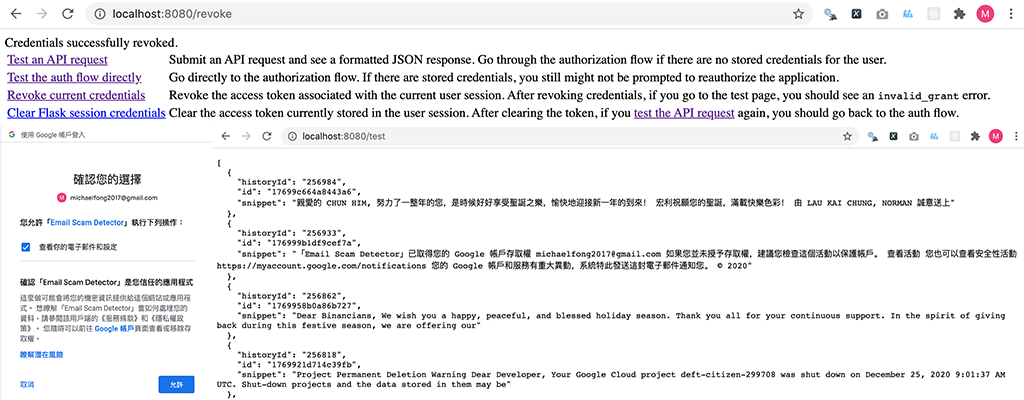
\includegraphics[width=0.7\columnwidth]{dev.png} % Example image
\end{center}

\noindent{The next step is to develop a Google Workspace add-on using the necessary Apps Script, giving the UI, behaviours and user interactions of the scam detector within the Gmail email client. This add-on interacts with the web server application via REST API. This add-on is listed, reviewed and published on the Google Workspace Marketplace.}

\section*{\large{4 \hspace{10pt} Scam detection}}
Email scams are basically phishing, where fake emails pretend to come from trusted organizations such as banks and online shops. They usually trick victims into going to a website with looks exactly like the real organization's website and then disclosing personal information. Other email scams can direct victim to a fraudulent online shop.
\textbf{The direct way} of scam detection is that for each incoming email, URLs and, if possible, URLs embedded in images are retrieved and searched in some database using a white list or black list.
\textbf{An efficient way} is to use machine learning, which integrates URL text features, domain name features and web content features to classify phishing or fraudulent websites. URL text features and domain name features are extracted from words that compose a URL based on query data from search engines like Google. Web content features include the number of repetitive paragraphs for online shops.
\textbf{A more innovative way} is to use NLP to determine the associated organization (e.g. Bank of East Asia) of the email and search whether the sender of the email is possible (e.g. whether it ends with @hkbea.com).

\end{document}